% !TEX root = thesis.tex
\startchapter{Meet IBM Rational Team Concert}
\label{chap:rtc}
In this chapter we describe the IBM Rational Team Concert\footnote{https://www.jazz.net} product as well as its development team,
since most of the research carried out throughout this thesis was in collaboration with this product development team which as part of their development process is also using their own product.
We begin with introducing the product and its functionalities before we describe the development team's composition and development process.

\section{The IBM Rational Team Concert Product}
IBM Rational Team Concert (RTC) is a server client application meant to support software development.
It is comprised of four major functionalities that bear relevance to this thesis:
(1) source control management that is based on similar principles as GIT\footnote{http://GIT-scm.com/} and mercurial\footnote{http://mercurial.selenic.com/}, (2) work item management to keep track of issues, tasks and features that need to be resolved and implemented, (3) planning capabilities to organize work items into iterations working towards milestones, and (4) a build engine that allows for continues builds and regression tests.

\subsection{Source Control}
\begin{figure}
\centering
\subfloat[A set of changes that is only on the developers local machine.]{\label{subfig:csb}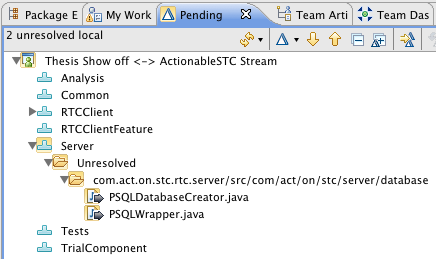
\includegraphics[width=.6\textwidth]{figures/meet-rtc.tex/change-before-set}}

\subfloat[A change-set that is also in the developers remote workspace.]{\label{subfig:cs}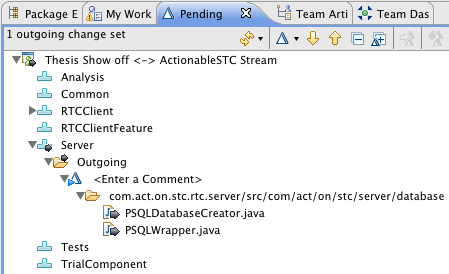
\includegraphics[width=.6\textwidth]{figures/meet-rtc.tex/change-set}}

\subfloat[A change-set that is attached to a work item.]{\label{subfig:csa}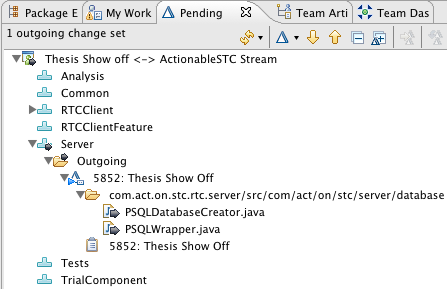
\includegraphics[width=.6\textwidth]{figures/meet-rtc.tex/change-after-set}}
\caption{From having created local changes over adding them to the remote workspace to attaching it to a work item.}
\label{fig:change-set}
\end{figure}

The source control system provided by Rational Team Concert is server based similarly to traditional version control systems such as CVS\footnote{http://www.nongnu.org/cvs} and SVN\footnote{http://subversion.tigris.org/}.
Yet, each developer has their own workspaces similarly to a local GIT or mercurial repository.
These branches or in RTC terminology streams can contribute their changes in the form of change-sets to other streams shared by teams or can be exchanged between workspaces.

With this the main difference between the RTC source code management system and a distributed source code management systems such as GIT lies with all the repositories or streams being present on one single machine as opposed to many different machines.
Even branching and sharing of changes to the source code work similarly to distributed version control systems as they can be freely moved in-between workspaces, in-between streams, and between streams and work spaces.

For example Figure~\ref{fig:change-set} presents a typical work flow after a unit of work has been finished and needs to be finalized.
A developer would gather all the changes that are only available on her local machine (Figure~\ref{subfig:csb}) and combine them into a change-set (Figure~\ref{subfig:cs}) that is at that point made available on her remote workspace.
After ideally linking that change-set to the task it is meant to resolve (Figure~\ref{subfig:csa}) the developer can deliver the change-set to the team stream to make it available to the whole team.

\subsection{Work Items}
\begin{figure}
\centering
\subfloat[A work item as most developer look at it from within the Eclipse client.]{\label{subfig:wieclipse}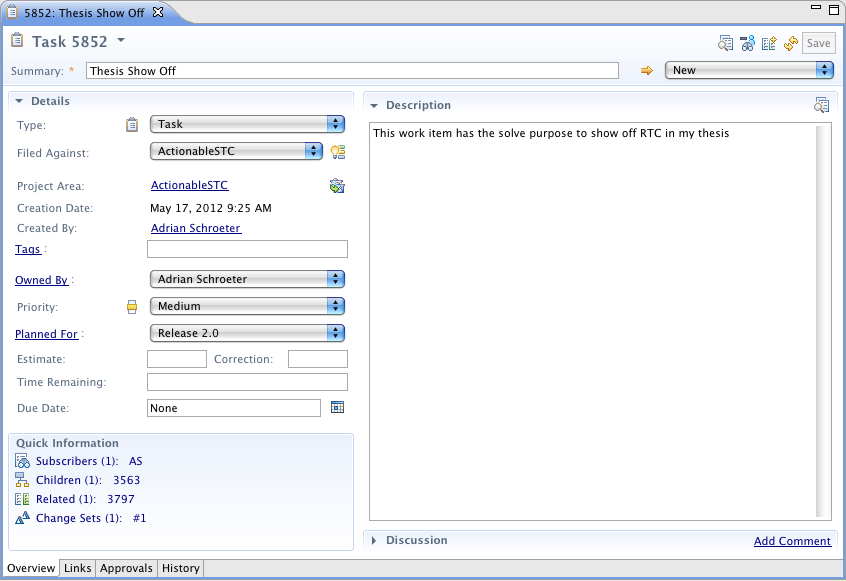
\includegraphics[width=\textwidth]{figures/meet-rtc.tex/wi-eclipse}}

\subfloat[A work item as most manager look at it from the web ui.]{\label{subfig:wiweb}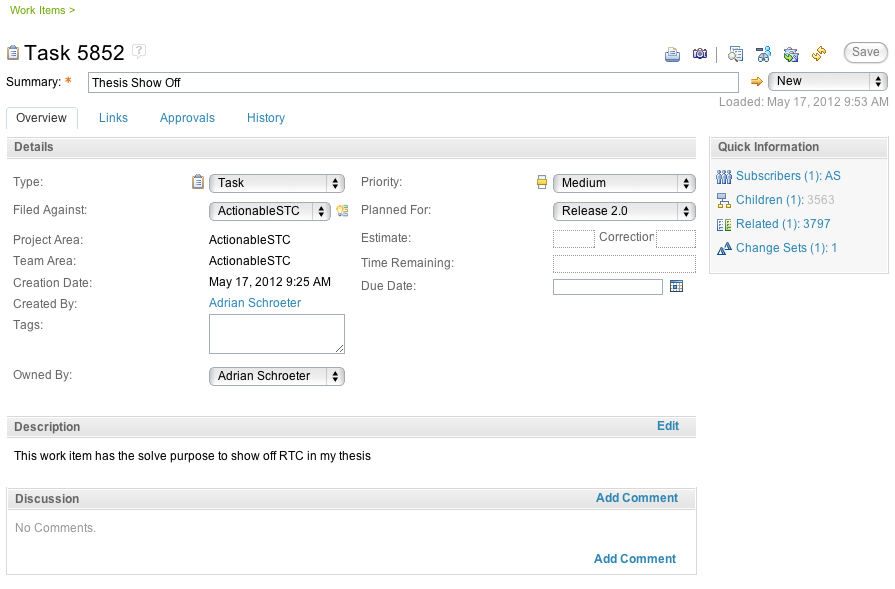
\includegraphics[width=\textwidth]{figures/meet-rtc.tex/wi-web}}
\caption{Workitems as shown by the different RTC UI's.}
\label{fig:wi}
\end{figure}
The work item component serves two functions: (1) it allows for customer interaction as it allows a customer or user to file feature requests and file bug reports and (2) it allows developers to manage their work by creating tasks as well as discuss and document thoughts about a defined unit of work.
These work items are basically an extension to bug reports as filed to a Bugzilla\footnote{http://www.bugzilla.org/}, since they serve more purposes than capturing bug reports and feature requests.

Developers have the ability to link work items into logical units and build hierarchies of work items to structure their work.
Furthermore, work items allow tracking meta information, such as time estimates, severity, and priority, and on top of that lends themselves to be customized with self defined fields on a project configuration level.
For example in Figure~\ref{fig:wi} we see the work item view from within Eclipse (Figure~\ref{subfig:wieclipse}) and through the web (Figure~\ref{subfig:wiweb}).
Both representations show links to other work items in the Quick Information pane as well as links to other artifacts such as change-sets.

\subsection{Planning}
\begin{figure}[t]
\centering
\subfloat[Planning from the Eclipse UI.]{\label{subfig:planeclipse}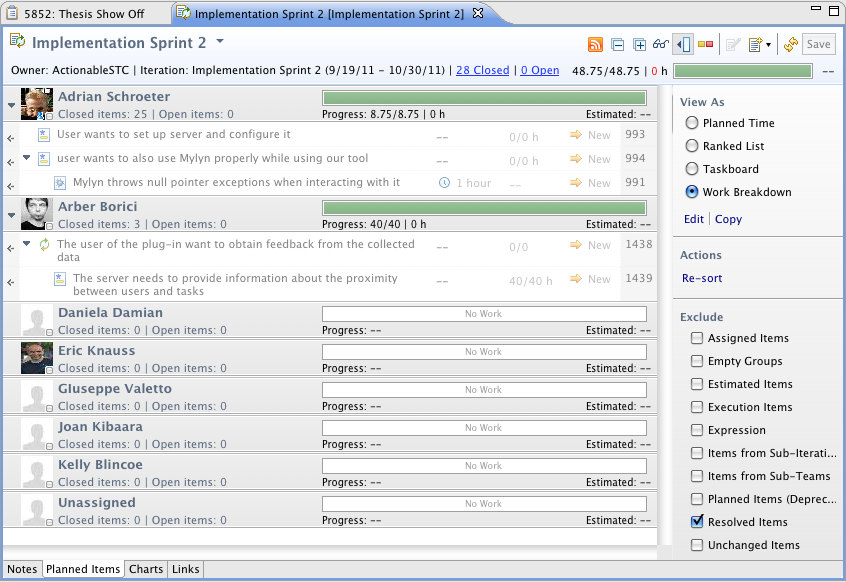
\includegraphics[width=.48\textwidth]{figures/meet-rtc.tex/plan-eclipse}\hspace{10pt}}
\subfloat[Planning from the Web UI.]{\label{subfig:planweb}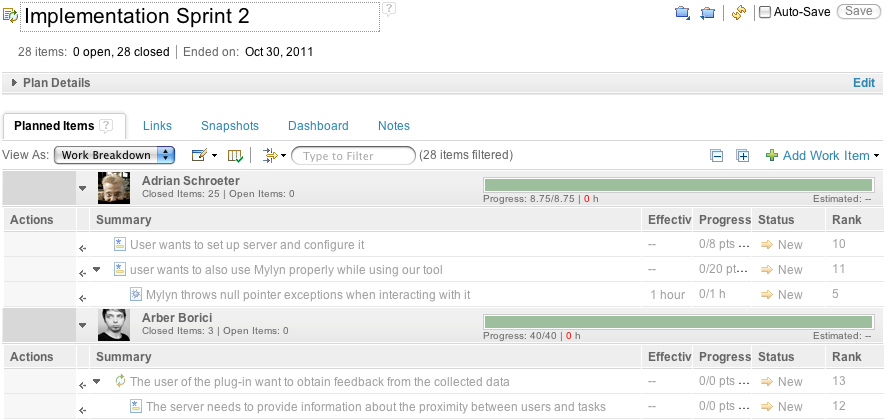
\includegraphics[width=.48\textwidth]{figures/meet-rtc.tex/plan-web}}
\caption{Plans as shown by the different RTC UI's.}
\label{fig:plan}
\end{figure}
\begin{figure}[t]
\centering
\subfloat[Chars in the Eclipse UI.]{\label{subfig:charteclipse}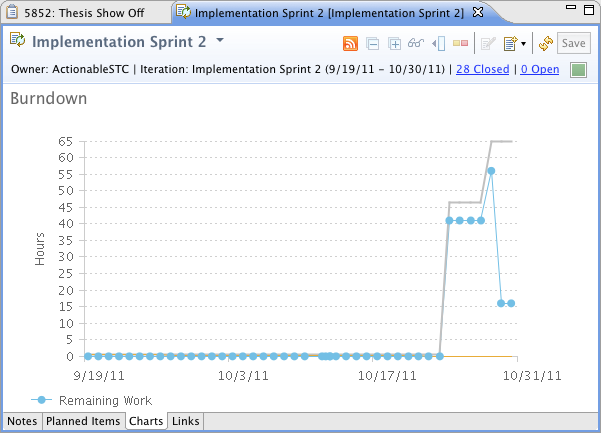
\includegraphics[width=.48\textwidth]{figures/meet-rtc.tex/chart-eclipse}\hspace{10pt}}
\subfloat[Chars in the Web UI.]{\label{subfig:chartweb}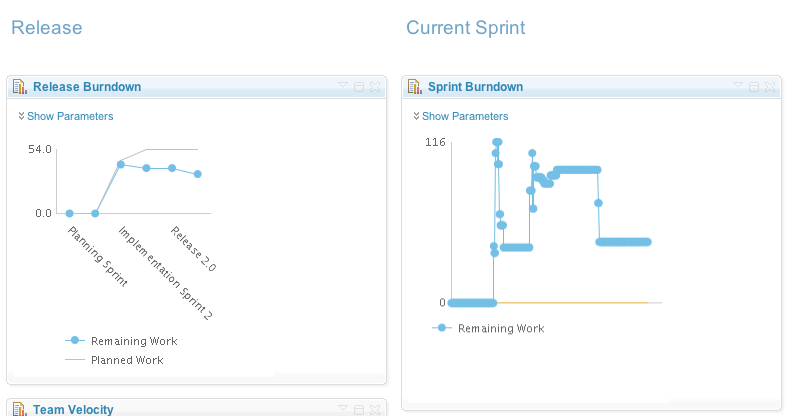
\includegraphics[width=.48\textwidth]{figures/meet-rtc.tex/chart-web}}
\caption{Charts as shown by the different RTC UI's.}
\label{fig:charts}
\end{figure}
In contrast to issue trackers such as bugzilla IBM Rational Team Concert offers planning capabilities.
Within RTC plans can be defined that consists of a number of work items that can be ranked against each other and assigned to different team members (see Figure~\ref{fig:plan} for an example).
RTC also supports multiple plans for different teams to support a better overview for the teams instead of cluttering plans with less relevant tasks.

The planning component supports several development styles reaching from agile-development styles such as XP and SCRUM~\cite{larman:ieeecomputer:2003} to more traditional development methods such as Waterfall~\cite{boehm:senotes:1986}.
Each different development style comes with a different default of control measures and charts such as burn down charts.
These charts as well as the planning can be both reviewed in the Eclipse and web client.
Both can be viewed in a customizable dashboard for quick information retrieval to stay up to date.
Figure~\ref{fig:charts} shows some examples of burn down charts as they show up on the Eclipse client (Figure~\ref{subfig:charteclipse}) and the Web UI (Figure~\ref{subfig:chartweb}).

\subsection{Build Engine}
The RTC build engine is comparable to build engines such as IBM Rational Buildforge\footnote{http://www-01.ibm.com/software/awdtools/buildforge/enterprise/} and Jenkins\footnote{http://jenkins-ci.org/}.
As build engine it allows for both, automated builds in pre-defined intervals such as nightly builds as well as on demand builds from users.
Build Results RTC can either be \error, \texttt{WARNING} or \ok. 

\subsection{Foundation/Integration}
\begin{figure}[t]
\centering
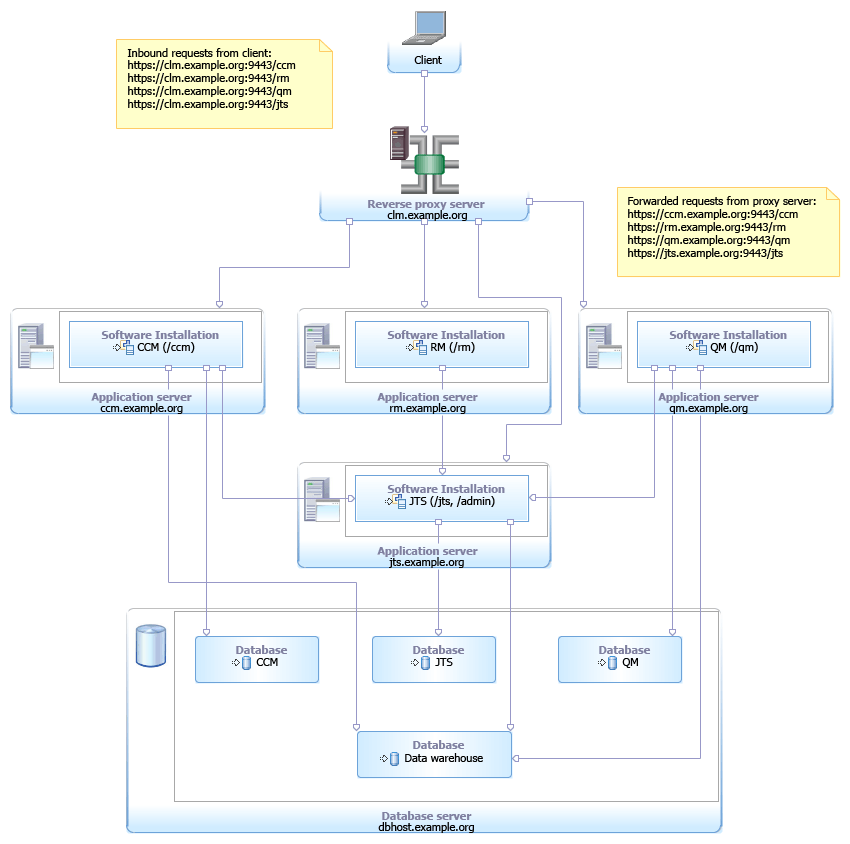
\includegraphics[width=.8\textwidth]{figures/meet-rtc.tex/rtc-topology}
\caption{RTC topology}
\label{fig:rtctopology}
\end{figure}
The IBM Jazz Foundation builds the layer on which the previously described components run.
By itself it does not offer any capabilities to the user, but it enables each component to integrated with the others. 
This allows the developer to both manually link artifacts with each other and define queries that cross reference multiple repositories.
Figure~\ref{fig:rtctopology} shows the three layers of the RTC product.
At the top is the user that interacts with the application servers, ranging from source control over planing to work item management.
These application run on a common platform on the bottom also referred to as the Jazz Foundation server which runs onto a database instance.

For example, a developer is working on implementing a work item and create changes to the code base that he bundles into a change-set.
Before she submits the change-set resolving the work item she links that change-set to the work item.
This enables her colleagues to easily accept the change-set into their workspaces to both review and test them.
Once the work item is resolved, the plan and the burn-down charts update to reflect this change visible to anyone with access to the plan and charts.

Developers often need to modify existing code and therefore need to understand the thought process that went into the code they are looking at~\cite{vonmayrhauser:ieeecomputer:1995}.
For this purpose developers can create queries that look for work items associated with changes to this code parts and instead of reading source code, they have access to documentation related to the code they are investigating.


\section{The IBM Rational Team Concert Product Development Team}
The IBM Rational Team Concert product development team is distributed across multiple sites following an agile development methodology.
In this section we are going to characterize the development team at large as well as describing their development process.

\subsection{The People}
\begin{table}[t]
\centering
\begin{tabular}{r@{\hspace{20pt}}l@{\hspace{20pt}}l@{\hspace{20pt}}l@{\hspace{20pt}}l}
\toprule
&total& minimum & maximum& average\\
\midrule
Number of Locations &  $>$16\\
Number of Teams & 47\\
Number of Developers & 151\\
Range of Team size & & 1& 20 & 5.7\\
Range of Developer per Location & & 7 & 24 & 14.8\\
\bottomrule
\end{tabular}
\caption{Descriptive statistics of Rational Team Concert development team.}
\label{tab:teamstats}
\end{table}

\begin{figure}[t]
\begin{center}
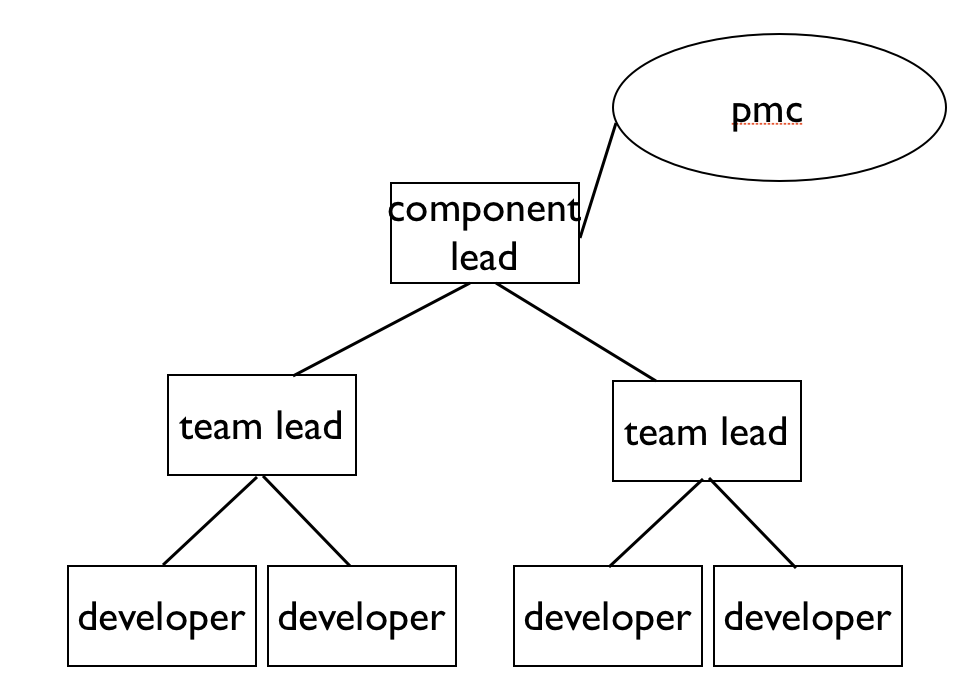
\includegraphics[width=.8\textwidth]{figures/meet-rtc.tex/ppl-orga}
\caption{Organizational structure of the technical personal in the RTC development team.}
\label{fig:orgastruct}
\end{center}
\end{figure}

The Rational Team Concert team is a large distributed team and uses the Rational Team Cocert for development. 
The Rational Team Concert development involves distributed collaboration over 16 different sites located in the United States, Canada, and Europe. 
Seven sites are active in RTC development and testing. 
There are 151 active contributors working in 47 teams at these locations, where contributors belong to multiple teams. 
Each team is responsible for developing a subsystem or component of RTC.
The team size ranges from 1 to 20 and has an average of 5.7 members. 
The number of developers per geographical site ranges from 7 to 24 and is 14.8 in average.
Table~\ref{tab:teamstats} summarizes the mentioned team statistics.

The teams are organized into larger component based teams as well as subcomponent and cross-component teams.
A developer can be part of multiple teams but usually is only part of one component teams.
Most teams are located in one location with some satellite members in different locations.

Teams on a component level represent a wealth of experiences that can range from standing veterans that did software development for several decades to fresh university graduates, with the occasional intern.
This variance in experience also reflects in the organizational structure.
The more experiences project members take leading roles ranging from teams leads to component leads and program management council roles (see Figure~\ref{fig:orgastruct}):
\begin{description}
\item[Team Leads] are still involved with daily development activities and usually have more development experience especially with the sub-component their team is developing and maintaining.
Additionally, team leads are both the first contact person when cross component issues arise that need to be discussed with other teams.
Note, that this is for the initiation of the cross team collaboration and to communicate the severity and the need for the other team to re-prioritize their work items.
\item[Component Leads] work together with multiple team leads and are responsible for the implementation of larger components such as the source code management component and do less development work than team leads.
\item[Council Members] deal with component crossing issues, such as architectural or process related issues.
They decide how components interact as well as what changes need to implemented to fulfill certain feature requests on a higher level.
Furthermore, council members also discuss how feasible the implementation of features with respect to the existing architecture is.
\end{description}
Of course there are still ``regular'' software developers that are less involved in cross-component issues unless they are part of a cross-component teams to implement a feature that is similar across several components.
In contrast to team leads, developers focus on their daily implementation work and interact with other developers mainly to resolve issues.

\begin{figure}[t]
\centering
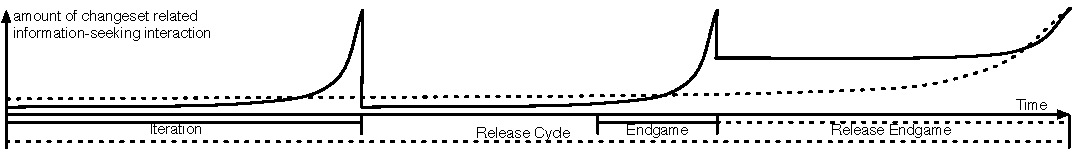
\includegraphics[width=\textwidth]{figures/findingProcess2}
\vspace{-20pt}\caption{The pattern of information-seeking interactions throughout several iterations of a release cycle. Every release cycle consists of a number of iterations; each iteration includes an endgame phase. change-set-based interactions are more frequent during endgame phases and during the last iteration of the release cycle.}
\label{IterationsFig1}
\end{figure}

\subsection{The Process}
\begin{figure}[t]
\begin{center}
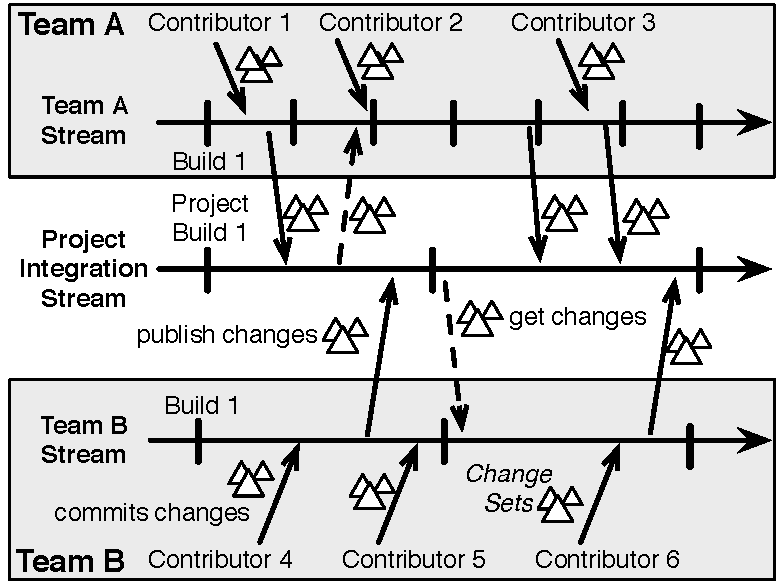
\includegraphics[width=.9\columnwidth]{figures/BuildResult}
\caption{Teams contribute to their own source streams, which are then merged into one project stream.}
\label{fig:buildresult1}
\end{center}
\end{figure}



The IBM Rational Team Concert development team follows an agile development methodology and high community involvement.
In short they are following the Eclipse Way of Development process describe by Frost~\cite{frost:ieeesoftware:2007}.
This development methodology places a large emphasis on community involvement.
Although IBM Rational Team Concert is not an open source product and non-employees are not given access to the actual source code repository the development team encourages the community to ask question on how to enrich both the server side components and the RTC client with additional plug-ins.

The development team progresses in six week iterations towards larger releases of IBM Rational Team Concert.
These iterations as well as the release cycle are further divided into end-game and non-end-game phases.
A typical release cycle begins with setting high level goals for the iteration to implement certain features that are determined by a committee (see Figure~\ref{IterationsFig1}).
These features represent a mix of customer, community, and developer suggestions, which are then formulated into user stories and epics for the release cycle.
These stories are then estimated and distributed across the six week iterations within a release cycles with a major milestone around the IBM Rational's Innovate conference\footnote{http://www.ibm.com/software/rational/innovate} to show case the latest version of IBM Rational Team Concert. 
At the end of each iteration the Rational Team Concert development team tries to switch to the latest RTC version for self-hosting in accordance to eating their own dog food for quality insurance.

On a day to day basis developers work on work items that are assigned to them by the team leads to work towards their iteration goals.
While working on a task developers document their thoughts on the respective work item and engage into discussions of work item related to their work.
Once the coding work for a work item is finished, a developer groups all changes into a change-set and attaches it to the respective work item and then delivers the change-set to the team stream.

Change-sets in the component team's stream are used to create nightly builds and run all the test cases on.
Once a build is stable for a component team, the change-sets provided by the team are bundled and distributed to the other component teams (see Figure~\ref{fig:buildresult1}).
During the non-end-game phase this process is very fluent and stream lined.
Once entering an endgame-phase the process of including change-sets into a build becomes more regulated.
Each change-set needs approval before it is included in a build.
Moreover, before a developer can start working on a work item its risk to the project and value needs to be assessed before a developer is allowed to start working on it.
